
\newcommand{\xxtheta}{f_\theta}
\section{문제 설정과 배경}
\label{sec:background}

먼저 제어 가능 생성을 정의하고(\cref{ssec:control_setup}), 이어서 연속 디퓨전 모델을 검토한다(\cref{ssec:diffusion_setup}).

\subsection{텍스트의 생성 모델과 제어 가능 생성}
\label{ssec:control_setup}
텍스트 생성은 학습된 언어모델 $\plm (\ww)$에서 $\ww$를 표집하는 과제이다. 여기서 $\ww = [w_1 \cdots w_n]$은 이산 단어 시퀀스이고, $\plm (\ww)$는 단어 시퀀스에 대한 확률분포이다. 제어 가능 텍스트 생성은 조건부 분포 $p(\ww \mid \cc)$에서 $\ww$를 표집하는 과제로, $\cc$는 \emph{제어(control)} 변수이다. 구문 제어에서 $\cc$는 목표 구문 트리(\cref{fig:1})일 수 있고, 감성 제어에서 $\cc$는 원하는 감성 라벨일 수 있다. 제어 가능 생성의 목표는 제어 목표 $\cc$를 만족하는 $\ww$를 생성하는 것이다.

플러그앤플레이 제어 가능 생성 설정을 고려하자. 대량의 비라벨 텍스트로 학습된 언어모델 $\plm(\ww)$가 주어지고, 각 제어 과제마다 적은 양의 라벨 텍스트로 학습된 분류기 $p(\cc \mid \ww)$가 주어진다(예: 구문 제어의 경우 분류기는 확률적 파서이다). 목표는 이 두 모델을 활용하여 베이즈 규칙 $p(\ww \mid \cc) \propto \plm(\ww) \cdot p(\cc \mid \ww)$를 통해 사후 $p(\ww \mid \cc)$에서 근사적으로 표집하는 것이다. 여기서 $\plm(\ww)$는 $\ww$가 유창하도록, $p(\cc \mid \ww)$는 $\ww$가 제어를 충족하도록 유도한다.






\subsection{자기회귀 언어모델}
언어모델링의 표준 접근은 $\plm$을 좌→우로 자기회귀 분해하는 것이다: $\plm(\ww) = \plm(w_1) \prod_{i=2}^n \plm(x_i \mid x_{<i})$. 이 경우 텍스트 생성은 지금까지 생성된 부분 시퀀스에 조건화하여 다음 토큰을 반복적으로 예측하는 과제로 환원된다. 다음 토큰 예측 $\plm(x_i \mid x_{<i})$는 보통 Transformer 아키텍처 \cite{Vaswani2017Attn}로 매개변수화된다.

\subsection{연속 영역의 디퓨전 모델}
\label{ssec:diffusion_setup}

디퓨전 모델 \citep{ho2020denoising,nichol2021improved}은 데이터 $\cx{0} \in \mathbb{R}^d$를 마르코프 사슬(Markov chain) $\cx{T} \dots \cx{0}$로 모델링하는 잠재변수 모델이며, 각 변수가 $\mathbb{R}^d$에 속하고 $\cx{T}$는 가우시안이다. 디퓨전 모델은 잠재변수 시퀀스 $\cx{T:1}$을 점진적으로 디노이징하여 목표 데이터 분포의 표본을 근사한다(\cref{fig:graphical_model}). 초기 상태는 $p_\theta(\cx{T}) \approx \mathcal{N} (0, \mathbf{I})$이고, 각 디노이징 전이 $\cx{t} \rightarrow \cx{t-1}$는 모델 $\ptheta(\cx{t-1}\mid \cx{t}) = \mathcal{N}(\cx{t-1}; \mu_\theta(\cx{t}, t), \Sigma_\theta(\cx{t}, t))$로 매개변수화된다. 예를 들어 $\mu_\theta$, $\Sigma_\theta$는 U-Net이나 Transformer로 계산될 수 있다.


디퓨전 모델을 학습하기 위해, 중간 잠재변수 $\cx{1:T}$를 구성하는 정방향(forward) 과정을 정의한다. 정방향 과정은 데이터 $\cx{0}$에 가우시안 노이즈를 점진적으로 더하여, 디퓨전 단계 $T$에서 표본 $\cx{T}$가 근사적으로 가우시안이 되도록 한다. 각 전이 $\cx{t-1} \rightarrow \cx{t}$는 $q(\cx{t} \mid \cx{t-1}) = \mathcal{N} (\cx{t} ; \sqrt{1-\beta_t} \cx{t-1}, \beta_t \mathbf{I})$로 매개변수화되며, 하이퍼파라미터 $\beta_t$는 디퓨전 단계 $t$에서 더해지는 노이즈 양이다.
정방향 과정 $q$의 매개변수화는 학습 가능한 파라미터를 포함하지 않으며, 이를 통해 사전 정의된 정방향 과정 $q$로 노이즈 데이터를 만들고 모델이 그 과정을 역으로 풀어 데이터를 재구성하도록 학습하는 학습 목적함수를 정의할 수 있다.




\begin{figure}
    \centering
    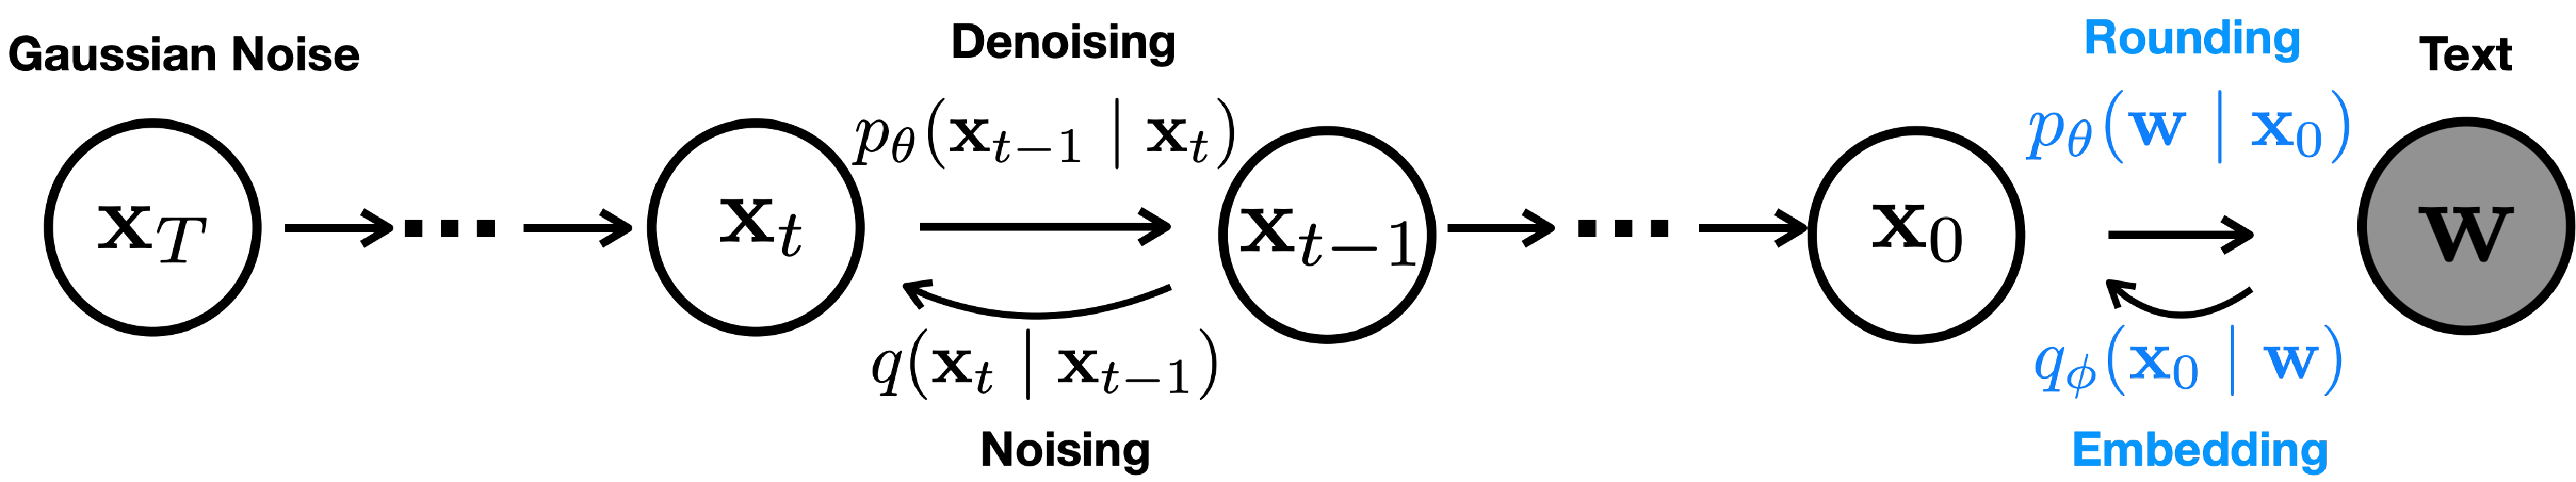
\includegraphics[width=0.8\textwidth]{fig/graphical_model_v2.pdf}
    \caption{\label{fig:graphical_model} 정방향·역방향 디퓨전 과정을 나타내는 그래픽 모델. 원래의 디퓨전 모델 \cite{ho2020denoising}에 더하여, 우리는 $\cx{0}$와 $\ww$ 사이에 마르코프 전이를 추가하고, 임베딩(\cref{ssec:embeddings})과 반올림(\cref{ssec:rounding}) 기법을 제안한다.}
    \vspace{-5mm}
\end{figure}

디퓨전 모델은 데이터의 주변 가능도 $\mathbb{E}_{\cx{0} \sim p_\text{data} }[\log p_\theta(\cx{0})]$를 최대화하도록 학습되며, 표준 목적함수는 $\log p_\theta(\cx{0})$의 변분 하한이다 \cite{pmlr-v37-sohl-dickstein15}.
\begin{equation}
\Lvlb (\cx{0}) = \mathop{\mathbb{E}}_{q(\cx{1:T} | \cx{0})} \left[\log \frac{q(\cx{T} | \cx{0})}{\ptheta(\cx{T})} + \sum_{t=2}^T \log \frac{q(\cx{t-1} | \cx{0},\cx{t})} {\ptheta(\cx{t-1} | \cx{t}) } - \log \ptheta( \cx{0} | \cx{1})\right].
\label{eqn:diffusion}
\end{equation}
하지만 이 목적함수는 불안정할 수 있고, 안정화에 많은 최적화 트릭을 필요로 한다 \cite{nichol2021improved}. 이 문제를 우회하기 위해 \citet{ho2020denoising}은 $\Lvlb$의 각 KL 발산 항을 전개·재가중하여 평균제곱오차 손실을 얻는 단순한 대리 목적함수를 고안했다(유도는 \cref{app:derive} 참조). 이를 다음과 같이 부른다.
\[\Lsimple (\cx{0}) = \sum_{t=1}^T \mathop{\mathbb{E}}_{q(\cx{t} \mid \cx{0})} || \mu_\theta(\cx{t}, t) - \hat{\mu}(\cx{t}, \cx{0}) ||^2,\]
여기서 $\hat{\mu}(\cx{t}, \cx{0})$는 닫힌 형식 가우시안인 사후 $q(\cx{t-1} | \cx{0},\cx{t})$의 평균이고, $\mu_\theta(\cx{t}, t)$는 신경망이 계산하는 $\ptheta(\cx{t-1} \mid \cx{t})$의 예측 평균이다.
$\Lsimple$은 더 이상 유효한 하한은 아니지만, 기존 연구에서 학습을 더 안정적으로 만들고 표본 품질을 향상시킨다고 경험적으로 보고되었다\footnote{우리의 $\Lsimple$ 정의는 \citet{ho2020denoising}과 다른 매개변수화를 사용한다. 우리는 제곱 손실을 $\mu_\theta(\cx{t}, t)$로 표현하지만 그들은 $\epsilon_\theta(\cx{t}, t)$로 표현한다.}.
Diffusion-LM에서도 학습 안정화와 표본 품질 향상을 위해 비슷한 단순화를 사용할 것이다(\cref{ssec:embeddings}).














\vspace{-2mm}
\section{Diffusion-LM: 연속 디퓨전 언어모델링}
\vspace{-2mm}
\label{sec:method}

Diffusion-LM 구성에는 표준 디퓨전 모델에 몇 가지 수정이 필요하다.
첫째, 이산 텍스트를 연속 공간으로 사상하는 임베딩 함수를 정의해야 한다. 이를 위해 임베딩을 학습하는 종단간 학습 목적함수를 제안한다(\cref{ssec:embeddings}).
둘째, 임베딩 공간의 벡터를 다시 단어로 사상하는 반올림 방법이 필요하다. 이를 위해 반올림을 돕는 학습 시·디코딩 시 방법을 제안한다(\cref{ssec:rounding}).








\vspace{-2mm}
\subsection{종단간 학습}
\label{ssec:embeddings}


이산 텍스트에 연속 디퓨전 모델을 적용하기 위해, 각 단어를 $\mathbb{R}^{d}$의 벡터로 사상하는 임베딩 함수 $\Emb(w_i)$를 정의한다. 길이 $n$ 시퀀스 $\ww$의 임베딩은 $\Emb(\ww) = [\Emb(w_1), \dots, \Emb(w_n)] \in \mathbb{R}^{nd}$로 정의한다.

식 \ref{eqn:diffusion}의 디퓨전 모델 학습 목적함수를 수정하여, 디퓨전 모델의 파라미터와 단어 임베딩을 함께 학습한다.
예비 실험에서 우리는 무작위 가우시안 임베딩과 사전학습 단어 임베딩 \cite{pennington-etal-2014-glove, radford2019language}을 모두 시도해 보았다. 이러한 고정 임베딩들은 종단간 학습에 비해 Diffusion-LM에 차선이라는 점을 발견했다\footnote{학습 가능한 임베딩이 제어·생성 과제에서 가장 좋지만, 어휘 단순체(simplex)로의 고정 임베딩이 홀드아웃 perplexity 최적화에는 도움이 됨을 확인했다. 본 연구의 초점은 perplexity가 아니라 생성 품질이므로 이 접근과 perplexity 결과의 논의는 \cref{app:simplex}로 미룬다.}.


그림 \ref{fig:graphical_model}처럼, 우리 접근은 정방향 과정에서 이산 단어 $\ww$로부터 $\cx{0}$로의 마르코프 전이를 추가하며, 이는 $\qphi(\cx{0} | \ww) = \mathcal{N} (\Emb(\ww), \sigma_0 I )$로 매개변수화된다. 역방향 과정에는 학습 가능한 반올림 단계를 추가하며, 이는 $\ptheta(\ww \mid \cx{0}) = \prod_{i=1}^n \ptheta(w_i \mid x_i)$로 매개변수화된다. 여기서 $\ptheta(w_i \mid x_i)$는 소프트맥스 분포이다. \cref{sec:background}에서 도입한 학습 목적함수는 이제 다음과 같아진다.
\begin{equation}
\begin{aligned}
\mathcal{L}^\text{e2e}_{\text{vlb}} (\ww) &= \mathop{\mathbb{E}}_{q_\phi(\cx{0} | \ww)}\left[\mathcal{L}_{\text{vlb}} (\cx{0}) + \log \qphi(\cx{0} | \ww) - \log \ptheta(\ww | \cx{0})]\right], \\
 \mathcal{L}^\text{e2e}_\text{simple} (\ww) &= \mathop{\mathbb{E}}_{\qphi(\cx{0:T} | \ww)} \left[\Lsimple(\cx{0}) + || \Emb(\ww) - \mu_\theta(\cx{1}, 1) ||^2  - \log \ptheta(\ww | \cx{0})\right].
\end{aligned}
\label{obj:e2e}
\end{equation}
\begin{wrapfigure}[11]{R}{0.5\textwidth}
\vspace{-10mm}
\centering
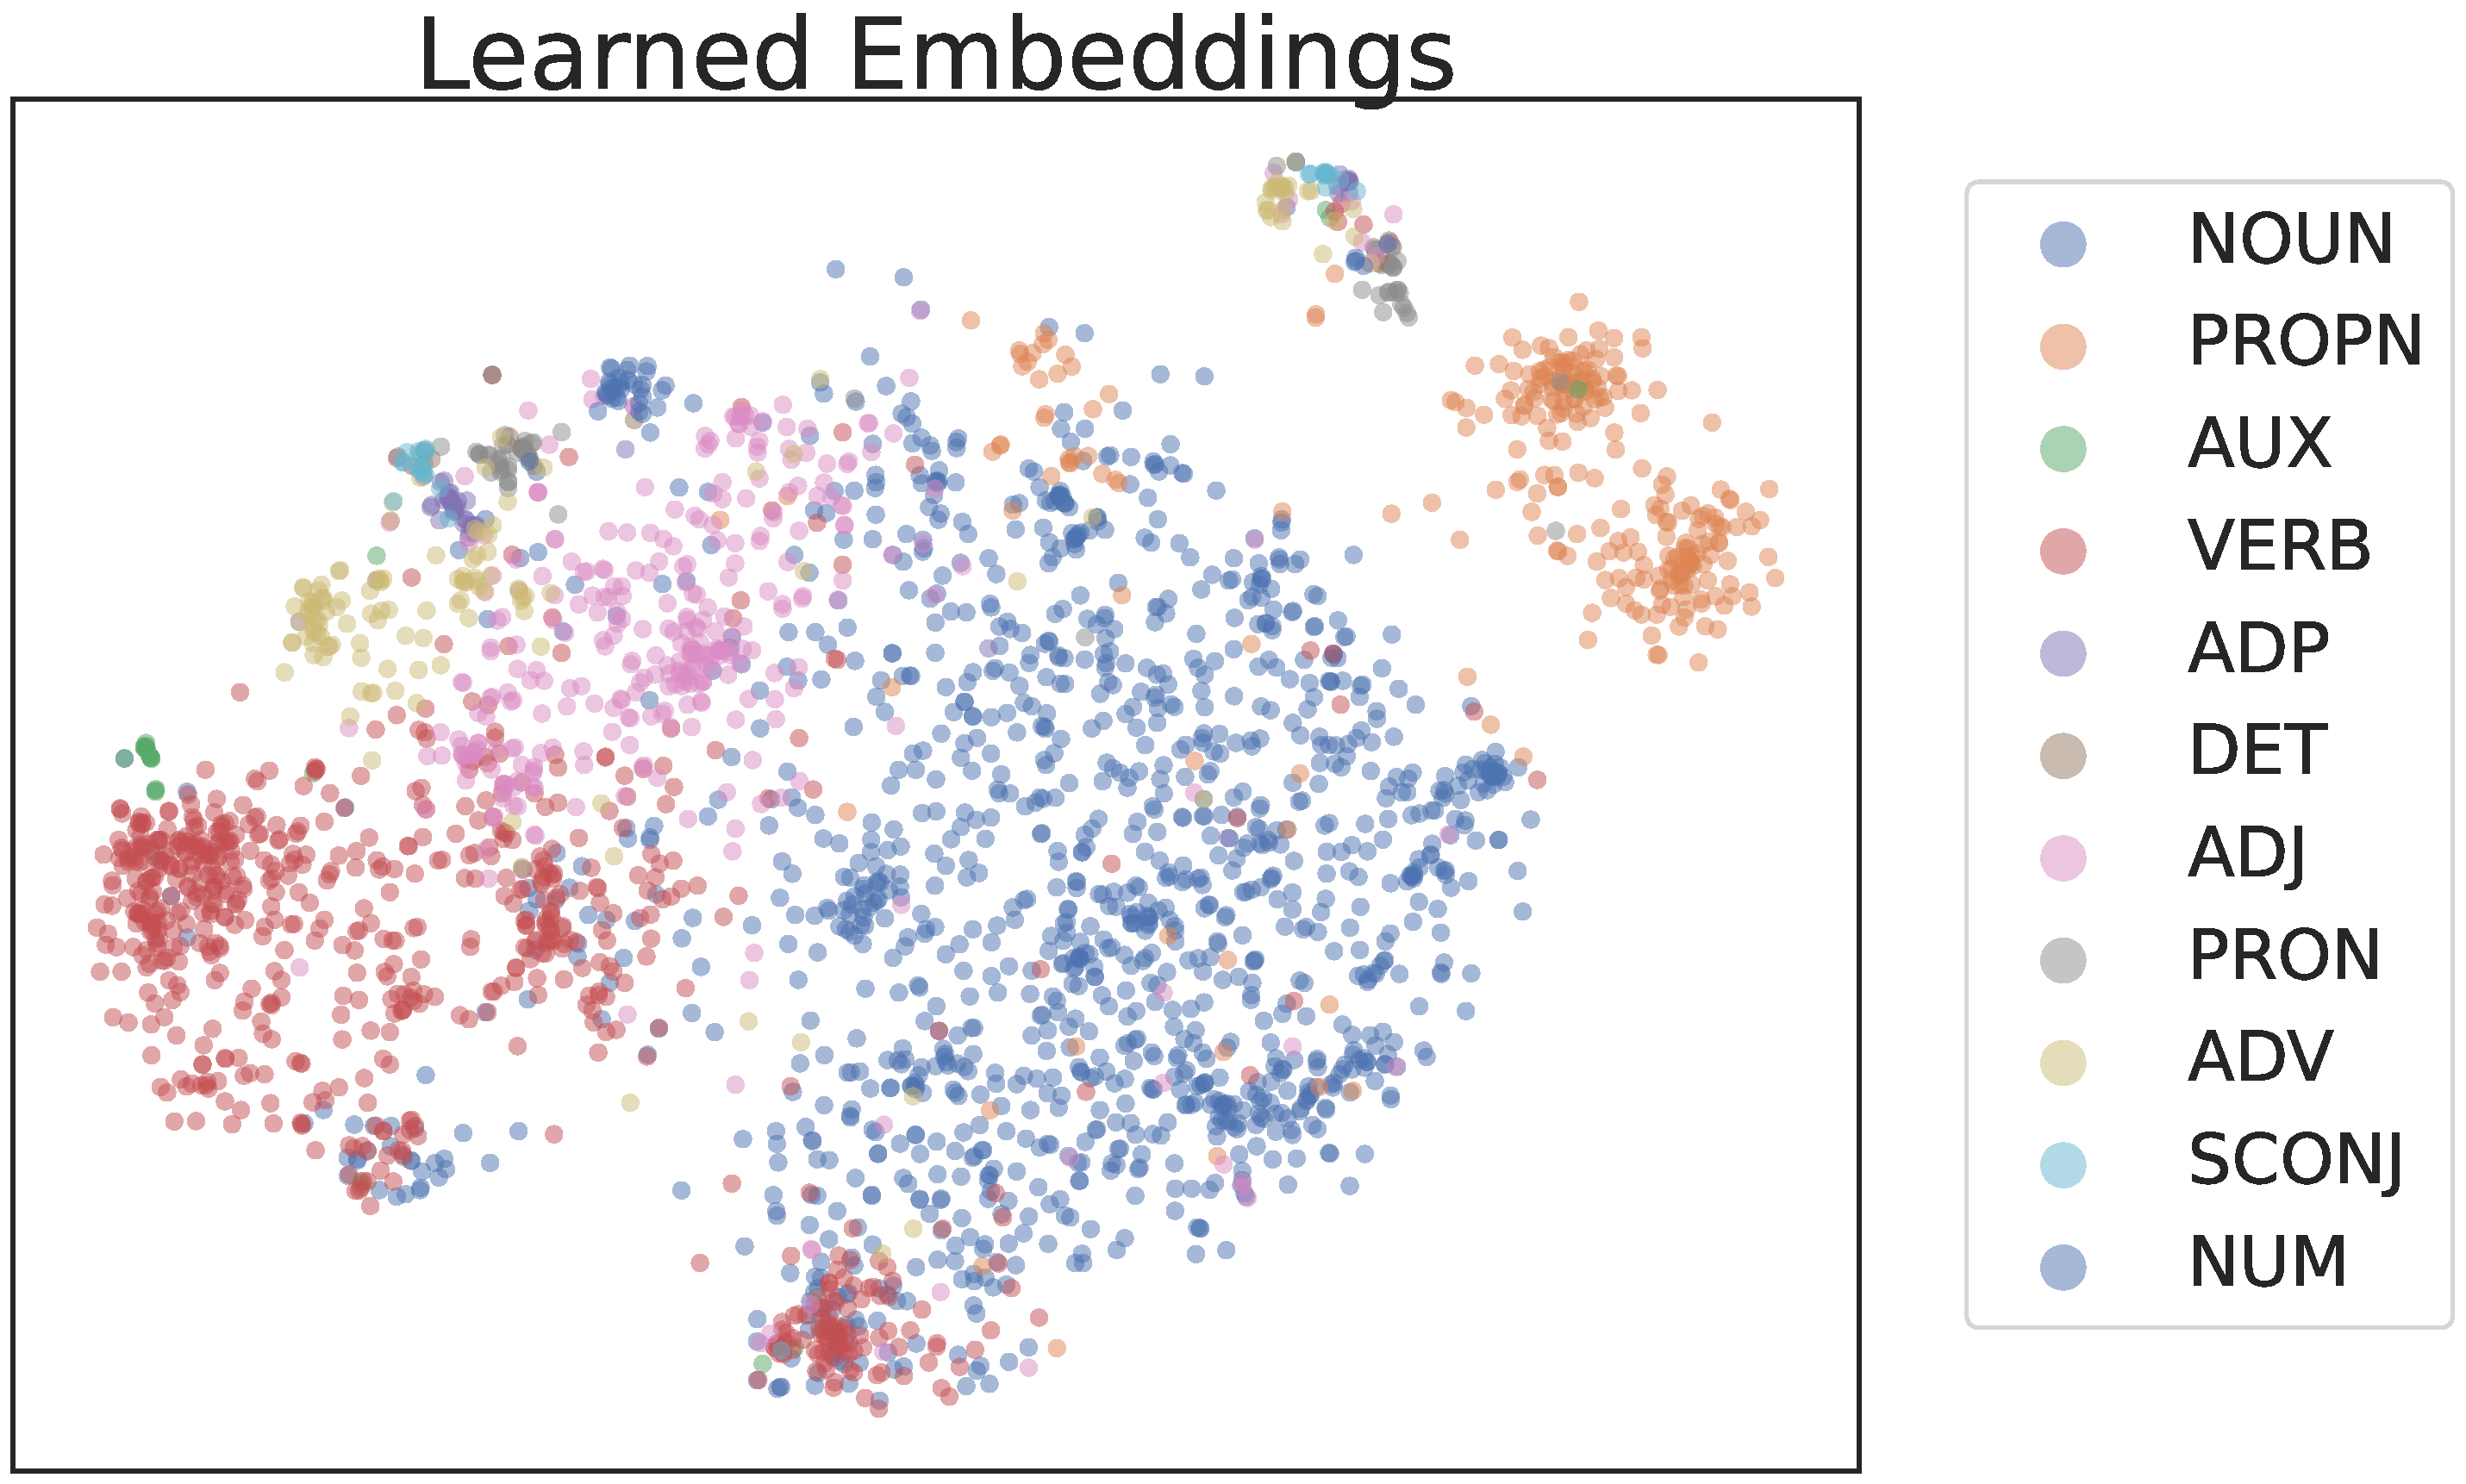
\includegraphics[width=\linewidth]{fig/embedding_128_v3.pdf}\caption{ \label{fig:emb} 학습된 단어 임베딩의 t-SNE \cite{vanDerMaaten2008} 도식. 각 단어는 그 품사로 색칠되어 있다. \looseness=-1 }
\end{wrapfigure}

$ \mathcal{L}^\text{e2e}_\text{simple} (\ww)$은 \cref{ssec:diffusion_setup}의 단순화를 따라 $\mathcal{L}^\text{e2e}_{\text{vlb}}(\ww)$로부터 유도하며, 자세한 유도는 \cref{app:derive}에 있다. 우리는 임베딩 함수를 학습하므로 이제 $q_\phi$가 학습 가능한 파라미터를 포함하며, 이 표집 단계를 통과하여 역전파하기 위해 재매개변수화 트릭 \citep{rezende2014stochastic, kingma2014auto}을 사용한다.
경험적으로 학습된 임베딩이 의미 있게 군집을 이룸을 확인했다. 같은 품사 태그(구문 역할)를 가진 단어들이 군집을 이루는 경향이 있으며, 이는 \cref{fig:emb}에 나타나 있다.



\subsection{반올림 오차 줄이기}
\label{ssec:rounding}


학습된 임베딩은 이산 텍스트에서 연속 $\cx{0}$로의 사상을 정의한다. 이제 예측된 $\cx{0}$를 다시 이산 텍스트로 반올림하는 역과정을 설명한다. 반올림은 위치마다 $\ptheta(\ww \mid \cx{0})= \prod_{i=1}^n \ptheta(w_i \mid x_i)$의 argmax에 따라 가장 확률이 높은 단어를 선택해 이루어진다. 이상적으로는 디노이징 단계가 $\cx{0}$를 어떤 단어의 임베딩 위에 정확히 놓이게 보장하기 때문에 argmax 반올림만으로 이산 텍스트로 사상하기에 충분해야 한다. 그러나 경험적으로 모델은 단일 단어에 정착하는 $\cx{0}$를 생성하지 못한다.



이 현상의 한 가지 설명은, 우리의 목적함수 \ref{obj:e2e}에서 $\Lsimple(\cx{0})$ 항이 $\cx{0}$의 구조를 모델링하는 데 충분히 무게를 두지 않는다는 것이다. $\Lsimple(\cx{0}) =\sum_{t=1}^T \mathbb{E}_{\cx{t}}|| \mu_\theta(\cx{t}, t) - \hat{\mu}(\cx{t}, \cx{0}) ||^2$의 정의를 떠올려 보자. 우리 모델 $\mu_\theta(\cx{t}, t)$는 디노이징 단계 $t$마다 $\ptheta(\cx{t-1}\mid \cx{t})$의 평균을 직접 예측한다.
이 목적함수에서 $\cx{0}$가 단일 단어 임베딩에 정착해야 한다는 제약은 $t$가 0에 가까운 항에서만 나타나며, 이러한 매개변수화는 그 항들을 강조하도록 목적함수를 신중하게 튜닝해야 함을 확인했다(\cref{app:ablation} 참고).


\newcommand{\Lsimplexx}{\mathcal{L}^\text{e2e}_{\cx{0}\text{-simple}}}
우리 접근은 $\Lsimple$을 재매개변수화하여 Diffusion-LM이 목적함수의 \emph{모든} 항에서 $\cx{0}$를 명시적으로 모델링하도록 강제한다. 구체적으로, $\cx{0}$로 매개변수화된 $\Lsimple$의 유사 형태인 $\Lsimplexx(\cx{0})=\sum_{t=1}^T \mathbb{E}_{\cx{t}} ||\xxtheta(\cx{t}, t) - \cx{0} ||^2$를 유도한다. 여기서 모델 $\xxtheta(\cx{t}, t)$는 $\cx{0}$를 직접 예측한다\footnote{$\cx{t-1}$의 분포는 정방향 과정 $\cx{t-1} = \sqrt{\alphabar} \cx{0} +\sqrt{1-\alphabar} \epsilon$로부터 닫힌 형식으로 얻을 수 있으므로, $\cx{0}$를 예측하는 것과 $\cx{t-1}$을 예측하는 것은 스케일링 상수까지 동치이다. 자세한 내용은 \cref{app:derive} 참고.}. 이는 신경망이 모든 항에서 $\cx{0}$를 예측하도록 강제하며, 이 목적함수로 학습한 모델은 $\cx{0}$가 단어 임베딩에 정확히 중심을 두어야 함을 빠르게 학습함을 확인했다.

위에서 모델 학습에 재매개변수화가 어떻게 도움이 되는지 설명했지만, 같은 직관을 디코딩 시에도 사용할 수 있는 기법이 있다. 이를 \emph{클램핑(clamping) 트릭}이라 부른다.
$\cx{0}$ 매개변수화 모델의 표준 생성 절차에서, 모델은 먼저 $\xxtheta(\cx{t}, t)$로 $\cx{0}$의 추정치를 계산한 뒤 이 추정치에 조건화하여 $\cx{t-1}$을 표집함으로써 $\cx{t}$를 $\cx{t-1}$로 디노이징한다: $\cx{t-1} = \sqrt{\alphabar} \xxtheta(\cx{t}, t) +\sqrt{1-\alphabar} \epsilon$, 여기서 $\alphabar_t = \prod_{s=0}^t (1-\beta_s)$, $\epsilon \sim \mathcal{N}(0,I)$\footnote{이는 모든 마르코프 전이가 가우시안이므로 닫힌 형식 가우시안이 되는 주변 분포 $q(\cx{t} \mid \cx{0})$로부터 따라 나온다.}. 클램핑 트릭에서는 모델이 추가로 예측 벡터 $\xxtheta(\cx{t}, t)$를 가장 가까운 단어 임베딩 시퀀스로 사상한다. 이제 표집 단계는 $\cx{t-1} = \sqrt{\alphabar}\cdot \Clamp(\xxtheta(\cx{t}, t)) +\sqrt{1-\alphabar} \epsilon$이 된다. 클램핑 트릭은 중간 디퓨전 단계의 예측 벡터가 단어에 정착하도록 강제하여 벡터 예측을 더 정확하게 만들고 반올림 오차를 줄인다.\footnote{직관적으로, $t$가 $T$에 가까운 초기 디퓨전 단계에 클램핑 트릭을 적용하는 것은 차선일 수 있다. 모델이 어떤 단어에 정착해야 할지 아직 결정하지 못했기 때문이다. 경험적으로 모든 디퓨전 단계에 클램핑 트릭을 적용해도 성능을 크게 해치지는 않는다. 다만 이 직관을 따르려면 클램핑 트릭의 시작 단계를 하이퍼파라미터로 둘 수도 있다.}


















\section{Diffusion-LM의 디코딩과 제어 가능 생성}
\label{sec:decode}
지금까지 Diffusion-LM을 설명했으며, 이제 제어 가능 텍스트 생성(\cref{ssec:control_text})과 디코딩(\cref{ssec:mbr1}) 문제를 다룬다.


\subsection{제어 가능 텍스트 생성}
\label{ssec:control_text}
이제 Diffusion-LM에서 플러그앤플레이 제어를 가능하게 하는 절차를 설명한다. \cref{ssec:control_setup}의 베이즈 정식화에서 영감을 얻되, 이산 텍스트에 직접 제어를 가하는 대신 Diffusion-LM이 정의하는 연속 잠재변수 시퀀스 $\cx{0:T}$에 제어를 가하고, 반올림 단계를 적용해 이 잠재변수들을 텍스트로 변환한다.

$\cx{0:T}$를 제어하는 일은 사후 $p(\cx{0:T} | \cc) = \prod_{t=1}^T p(\cx{t-1} \mid \cx{t}, \cc)$에서 디코딩하는 것과 동치이며, 이 결합 추론 문제를 각 디퓨전 단계의 제어 문제 시퀀스로 분해한다: $p(\cx{t-1} \mid \cx{t}, \cc) \propto p(\cx{t-1} \mid \cx{t}) \cdot p(\cc \mid \cx{t-1}, \cx{t})$.
이를 디퓨전 제어에 대한 기존 연구 \cite{song2021scorebased}의 조건부 독립 가정을 통해 $p(\cc \mid \cx{t-1}, \cx{t})=p(\cc \mid \cx{t-1})$로 더 단순화한다. 따라서 $t$번째 단계에서 우리는 $\cx{t-1}$에 대해 경사 갱신을 수행한다.
\begin{align*}
    \nabla_{\cx{t-1}} \log p(\cx{t-1} \mid \cx{t}, \cc) = \nabla_{\cx{t-1}} \log p(\cx{t-1} \mid \cx{t}) + \nabla_{\cx{t-1}}  \log  p(\cc \mid \cx{t-1}),
\end{align*}
여기서 $\log p(\cx{t-1} \mid \cx{t})$와 $\log p(\cc \mid \cx{t-1})$ 모두 미분 가능하다. 첫 항은 Diffusion-LM이 매개변수화하고, 두 번째 항은 신경망 분류기가 매개변수화한다.


이미지 영역의 연구 \cite{dhariwal2021diffusion,song2021scorebased}와 마찬가지로, 디퓨전 잠재변수에 대해 분류기를 학습하고 잠재 공간 $\cx{t-1}$에서 경사 갱신을 수행하여 제어를 충족하는 방향으로 유도한다. 이 이미지 디퓨전 연구들은 디퓨전 단계마다 $\nabla_{ \cx{t-1}} \log  p(\cc \mid \cx{t-1})$ 방향으로 한 번의 경사 단계를 취한다. 텍스트에서 성능을 높이고 디코딩을 가속하기 위해, 두 가지 핵심 변경을 도입한다: 유창성 정규화와 다중 경사 단계. \looseness=-1




유창한 텍스트를 생성하기 위해, \emph{유창성 정규화}가 포함된 제어 목적함수에 경사 갱신을 적용한다: $ \lambda \log p(\cx{t-1} \mid \cx{t}) + \log p(\cc \mid \cx{t-1})$. 여기서 $\lambda$는 유창성(첫 항)과 제어(둘째 항)를 절충하는 하이퍼파라미터이다. 디퓨전을 위한 기존 제어 가능 생성 방법은 목적함수에 $\lambda \log p(\cx{t-1} \mid \cx{t})$ 항을 포함하지 않지만, 이 항이 유창한 텍스트 생성에 결정적임을 확인했다. 이로 인한 제어 가능 생성 과정은 $p(\cx{t-1} \mid \cx{t}, \cc)$의 최대화와 표집 사이를 균형 짓는 확률적 디코딩 방법으로 볼 수 있으며, 이는 뉴클리어스 샘플링(nucleus sampling) \cite{Holtzman2020Nucleus}이나 낮은 온도(temperature) 샘플링 같은 텍스트 생성 기법과 비슷하다. 제어 품질을 높이기 위해 디퓨전 단계마다 다중 경사 단계를 취한다. 디퓨전 단계마다 Adagrad \footnote{Adagrad 대신 SGD를 사용하는 어블레이션도 시도했지만, Adagrad가 하이퍼파라미터 튜닝에 훨씬 덜 민감함을 확인했다.} \cite{Duchi2010AdaptiveSM} 갱신을 3 단계 수행한다. 늘어난 계산 비용을 완화하기 위해 디퓨전 단계 수를 2000에서 200으로 다운샘플링하면, 표본 품질을 크게 해치지 않으면서 제어 가능 생성 알고리즘이 가속된다.


\subsection{최소 베이즈 위험 디코딩}
\label{ssec:mbr1}
기계 번역이나 문장 채우기처럼 많은 조건부 텍스트 생성 과제는 \emph{단일} 고품질 출력 시퀀스를 요구한다.
이 환경에서, Diffusion-LM에서 표집한 샘플 집합 $\mathcal{S}$를 모은 뒤 손실함수 $\mathcal{L}$(예: 음의 BLEU 점수) 하에서 기대 위험을 최소화하는 샘플을 선택하는 최소 베이즈 위험(Minimum Bayes Risk, MBR) 디코딩 \cite{kumar-byrne-2004-minimum}을 적용한다: $\hat{\ww} = \argmin_{\ww \in S} \sum_{\ww' \in S} \frac{1}{|S|}\mathcal{L}(\ww, \ww')$. 저품질 샘플은 나머지 샘플들과 다르고 손실함수에 의해 패널티를 받기 때문에, MBR 디코딩이 흔히 고품질 출력을 반환함을 확인했다.





